
\section{スンマヘーン、500円になりまふぅ}
世紀の大捜査に終止符を打つため、我々は直接対決を申し込むことにしたのは前章までで述べたとおりである。
しかし、神戸から東京へ自費で行くにはあまりにもリスクがあったため、日本物理学会が宇都宮で開催されたタイミングで最終日に東京へ寄ることにしたのである。

本節では、直接対決までの前日譚を紹介し、いかに我々が本気で、問題解決へ挑んでいたかが分かっていただけることであろう。
以下では日本物理学会参加から、同期会、そして直接対決のため命をかけて東京へ行く様子を示す。

%全ては餃子の街、宇都宮が悪い。
%全ては我々を放り出し、中途半端に深夜3時ころに放り出した同期が悪い。
%全ては何かよく分からんラーメンを締めに食べた時間が悪い。
%全ては東京で海鮮食べ放題の店を見つけてしまった運命が悪い。

\section{直接対決へ向けた準備(食事面)}
竹田警部は以前にも東京へ単独での出張を行っており、たびたび東京でなにか面白いことはないかと調べていた所、
図\ref{fig:TaikoChaya}に行き着いた。
単独で乗り込むには少しハードルの高い、海鮮食べ放題の店であり、しかし兼ねてから機会を見つけては行きたいと感じていた。
そこに急遽、東京直接対決という機運が舞い込んできたため、さらに直接対決は午後からであることを鑑みて、たいこ茶屋に行くことができると判断した。
そこで、直接対決に同伴するオガワマンもたいこ茶屋参戦の提案を行い、海鮮好きな彼の了承も取り付けた。
直接対決への食事面に関する前準備は整ったのである。
たいこ茶屋で腹を満たし、すこし東京を観光し英気を養い、夕方からの対決へと挑む。
これが勝利への方程式であると確信した竹田警部は、しかし、驚愕の事実にぶち当たってしまう。
図\ref{fig:SeiriKen}を見ていただきたい。

\begin{figure}[htbp]
  \begin{center}
    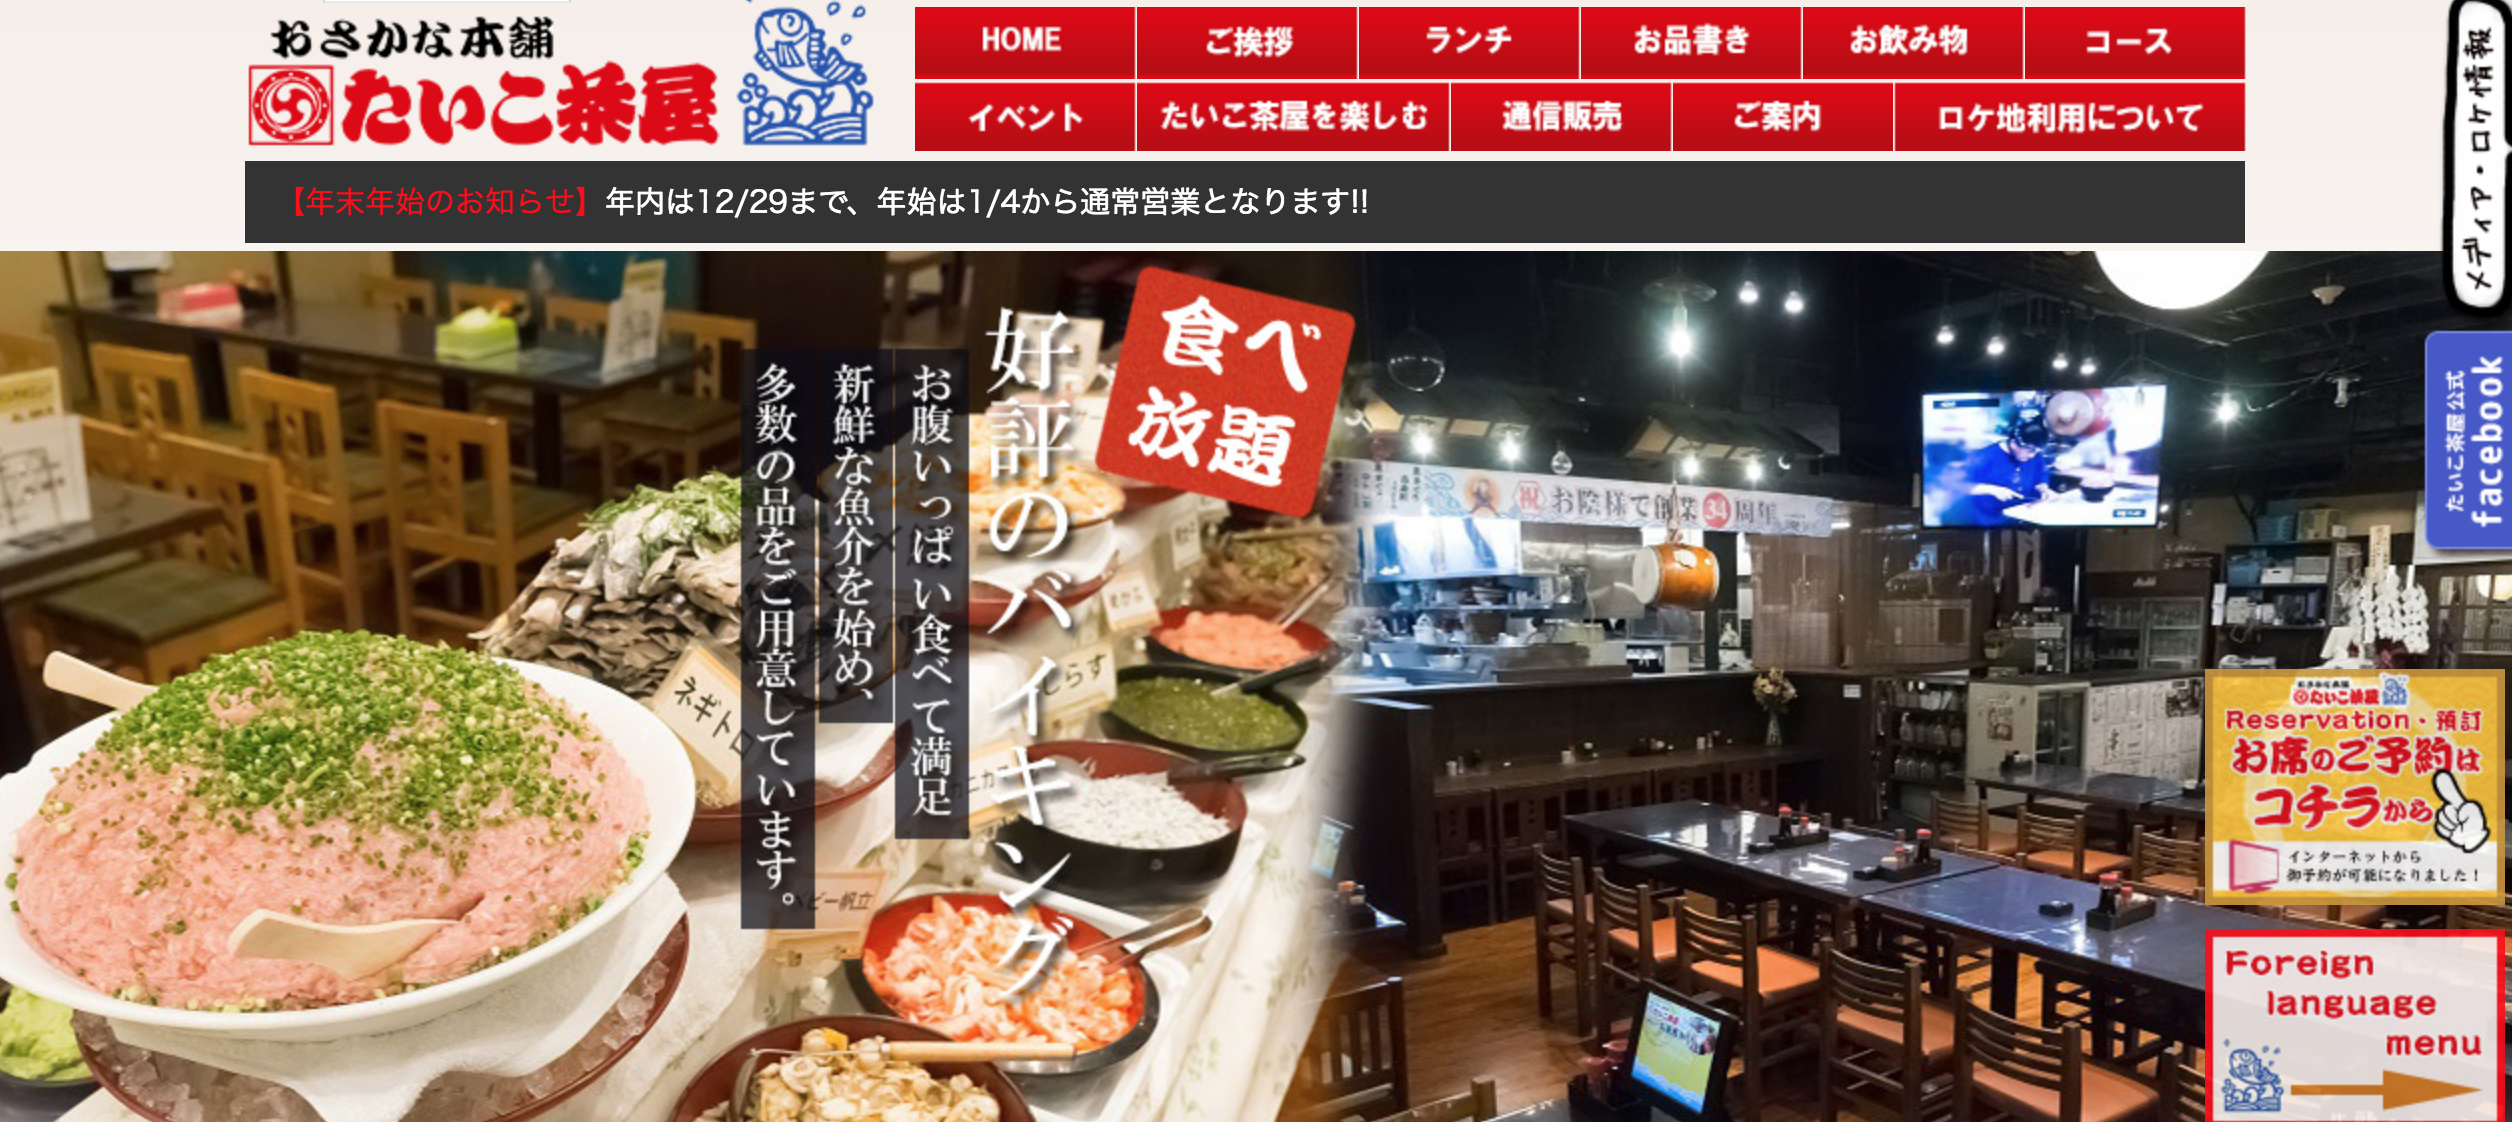
\includegraphics[width=0.7\textwidth]{./section/sasakiLIVE/figures/TaikoChaya.png}
  \end{center}
  \caption{東京の馬喰町にある、海鮮食べ放題の店。なんと整理券を貰わなければ入店することができないため、早朝から店頭に並ぶ必要がある様である}
  \label{fig:TaikoChaya}
\end{figure}

そう、このたいこ茶屋は整理券を配布し、一日の入場者に制限をかけているのである。
最新のスーパーコンピューター京のある神戸在住のオガワマンの持つiPhoneで検索した結果、
宇都宮から、東京の馬喰町に10時前に整理券配布の列に並ぶには、図\ref{fig:UmakuichoDensya}に示すように、7時起床が絶対的な条件となることがわかった。
ここから、学会最終日は早朝7時起床が義務付けられ、直接対決に向けた準備が粛々と進行していったのである。


\begin{figure}[htbp]
  \begin{center}
    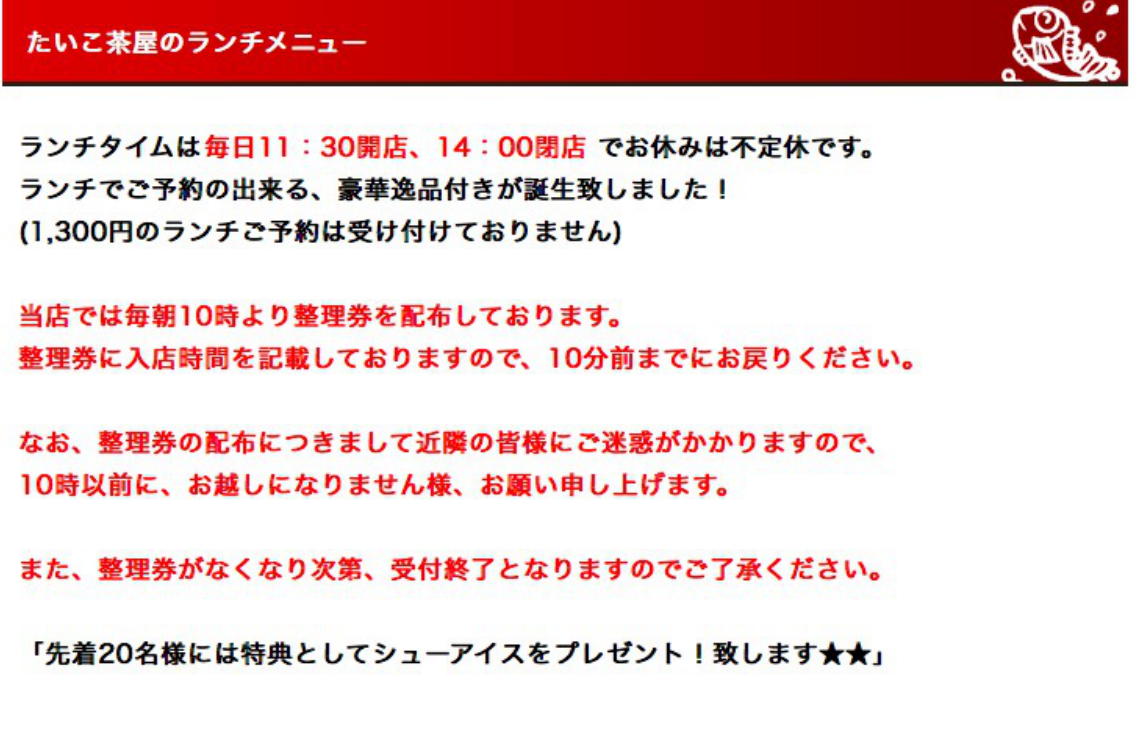
\includegraphics[width=0.6\textwidth]{./section/sasakiLIVE/figures/SeiriKen.png}
  \end{center}
  \caption{たいこ茶屋の整理券に関する情報。勝利への方程式を実現するには、なんとしても整理券を貰う必要があった。}
  \label{fig:SeiriKen}
\end{figure}

\begin{figure}[htbp]
  \begin{center}
    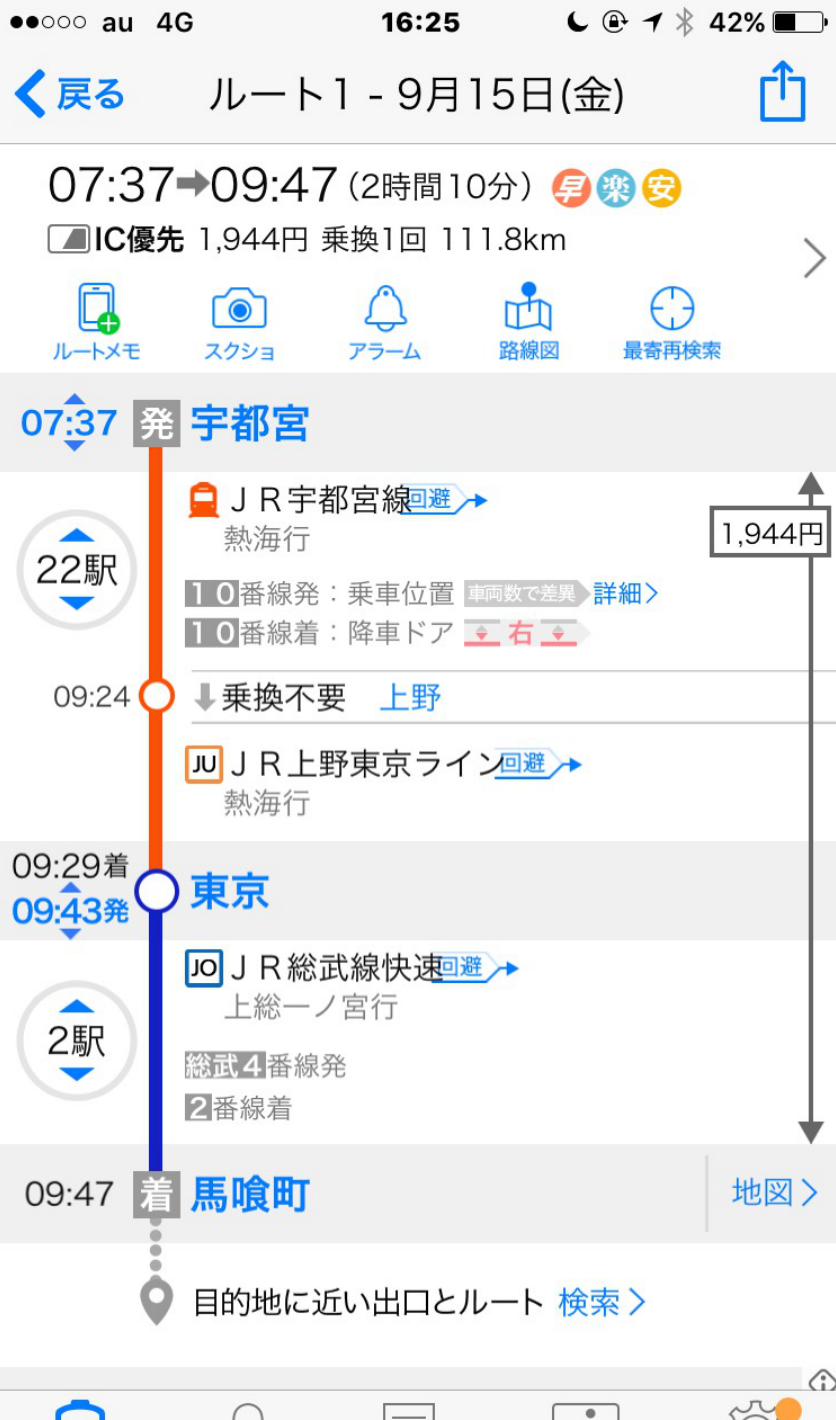
\includegraphics[width=0.4\textwidth]{./section/sasakiLIVE/figures/UmakuichoDensya.png}
  \end{center}
  \caption{10時前に馬喰町に降臨するには、宇都宮を7時半に出発する必要があり、7時には起床する必要があることが算出された。}
  \label{fig:UmakuichoDensya}
\end{figure}


\section{日本物理学会 2017年秋季大会}
2017年9月12日(火)〜15日(金)の期間、宇都宮大学峰キャンパスで日本物理学会が開催された。
ポマティは修士2年、修士課程最後の学会に挑んでいたのである。
期間中の夜には、日頃遠隔でのミーティング参加である研究グループの者同士が集まる懇親会が開かれていた。
9月14日に修士課程2年の同期が集まる飲み会が開催されることとなったのだが、なぜか竹田警部が運悪く、幹事になってしまったのである。
本来は幹事などしている場合ではない。
翌日15日の直接対決に向けて精神を研ぎ澄まし、今までに手に入れた証拠をもう一度洗い直し、我々の主張に問題がないことを確認しておかなければならないはずであった。
しかし、たしかに修士課程最後の学会ということもあり、就職してしまう同期に会えるのもこのタイミングしかないと思い、同期会開催には一定の意義もあったことはここで確認をしておきたい。
これが全ての始まりであった。
\par

急遽、同期の飲み会のためのLINEグループが立ち上がり、人数を募り、店を予約する、返事のない人間に個別でLINEを送り、などなど。
鬼の面倒である\footnote{その過程で、タニグバも誘ったのだが、来なかったという闇が存在している。}。
竹田警部はオガワマンにも声をかけ参加を募り、飲み会に消極的である彼を召喚することに成功したのである。
オガワマンにも参加して頂くことになったのであるが、図\ref{fig:OgawamanYaruki}に示すように、この時点では基本的に飲み会に消極的であり翌日の直接対決に向けた意思表明を行っている。
竹田警部も幹事という責務を果たしながら、図\ref{fig:TakedaYaruki}に示すように、翌日のためにもはや宿に帰らずオールナイトで起き続けるもしくはカラオケで仮眠をとるという、並々ならぬ意思表明を行っている。

\begin{figure}[htbp]
  \begin{center}
    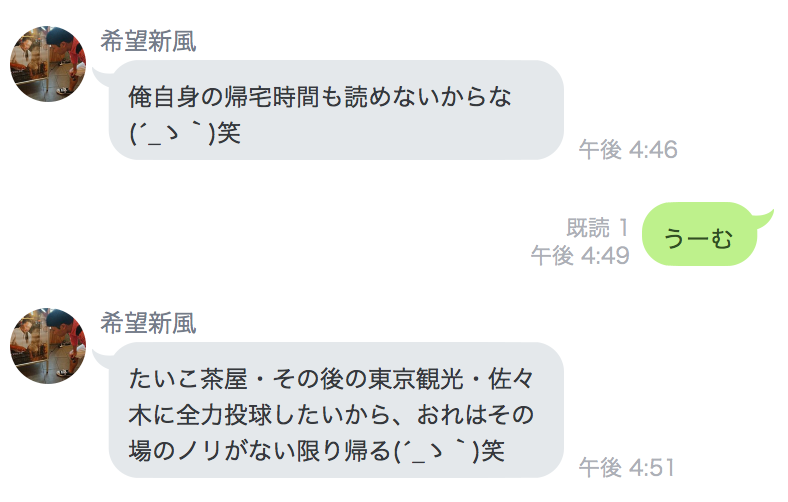
\includegraphics[width=0.5\textwidth]{./section/sasakiLIVE/figures/OgawamanYaruki.png}
  \end{center}
  \caption{オガワマンはぶれない男であり、飲み会は基本的に一次会で帰り翌日のイベント全てに全力投球をする旨の意思表明を行っている。この時点で竹田警部は幹事として飲み会が成功してほしいという気持ちが頭の中を支配しており、すこし温度差を感じる局面であった。}
  \label{fig:OgawamanYaruki}
\end{figure}

\begin{figure}[htbp]
  \begin{center}
    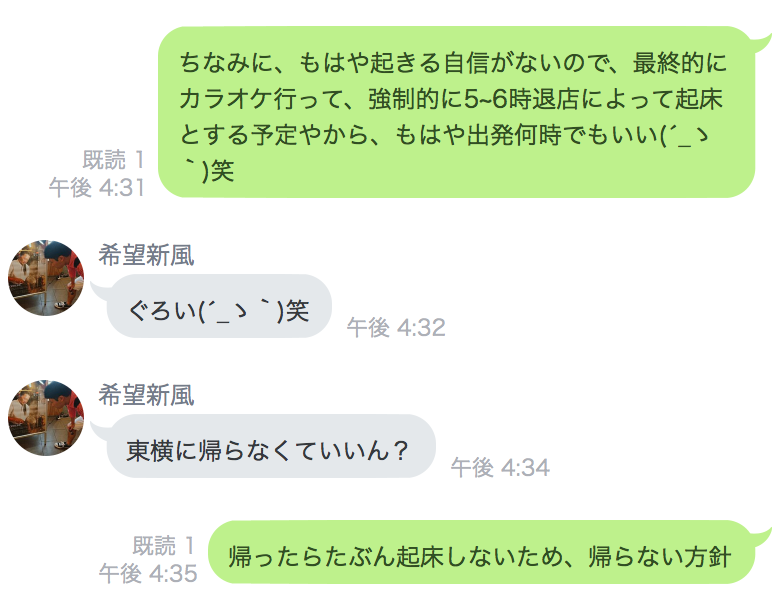
\includegraphics[width=0.5\textwidth]{./section/sasakiLIVE/figures/TakedaYaruki.png}
  \end{center}
  \caption{しかし、竹田警部も問題究明のために並々ならぬ覚悟を持って飲み会に参加する旨の意思表明を行っていることが過去のやり取りから見て取れる。}
  \label{fig:TakedaYaruki}
\end{figure}

補足説明を行うと、一次会に参加したオガワマンであったが、座った席の位置が非常に運が悪く鬼のようなメンツに囲まれて飲み会を進めていたようである(周りに日常会話のできる人間がおらず、気を抜けば物理の話しかしなかった状況)。
会の後半にはそのメンツからなんとか脱出をすることができたが、時すでに遅し。
虚しくも一次会終了のゴングが鳴ってしまったのである。
この時、竹田警部は「オガワマンにとって一次会は不発に終わってしまったかも知れない。二次会には来ないであろうな、、、 」と感じたそうである。

\par

しかし、奇跡が起きた。
翌日の直接対決へ向けたやる気が影響したのか、もしかすると不発に終わった一次会に不満を感じてしまったのか。
その理由や動機は今となっては定かではないが、なんとオガワマンが二次会参加表明を行ったのである。
これに勇気をもらった竹田警部は「よっしゃ二次会行くでぇ」と意気込み、もはや場所やどういう基準で選んだか覚えていないが、二次会の参加会場へと繰り出した\footnote{2次会にあの悪名高いミキザワナカティが参加していたような気がする。結局最後まで我々と完全には打ち解けなかった、ナゾの女性教師である。ちなみに、二次会は結構何喋ったか覚えてないが、後日ATLASの動機の前川くんに「このまえの同期会の二次会の竹田君はひどかった」とかなんとか言われた。また、会計をオガワマンにしてもらったのだが、なんか途中で帰ったか途中で来たか分からんややこしい人間が存在したために、計算を誤ってしまい1次会の浮いた分から会計が補填され事なきを得たことだけなんとなく覚えている。覚えている内容はそれくらい。}
盛り上がった二次会で会ったのであり、珍しく竹田・オガワ両名とも「このまま行くぞぉ」と意気込んでいたのであるが、なんと二次会終わりで皆が帰宅し、 二人が野に放たれてしまったのである。
このようなことが想像できたであろうか?
完全なる放送事故である。竹田警部はともかく、オガワマンが二次会まで参加し最後まで残っているのである。
普段は飲み会に消極的なオガワマンが翌日早朝7時起床でありながらも、覚悟を決め「これから」、という矢先に希望が断ち切られてしまったのである。

\section{野に放たれたポティの末路}
野に放たれた我々は宇都宮駅周辺で暴れまわったのである。
そのときの様子が克明に記録されている図を\ref{fig:OgawaPozu}、\ref{fig:Gyouza}に示す。
かくして我々は、おそらく当分くることの無いであろう宇都宮に大きな傷跡を残し、その夜の終止符を打ったのである\footnote{どうしようもなくなった我々は、締めのためにラーメンと餃子を食べに夜の街へと最後の気力を振り絞り繰り出すこととなった。その際にキャッチーとして近づいてきた女性に対し、その誘いを断っただけでなく「おすすめのラーメンないっすか?」と逆転の発想を繰り出し、無事最後の晩餐へとありつけたようである。}。

\begin{figure}[htbp]
  \begin{center}
    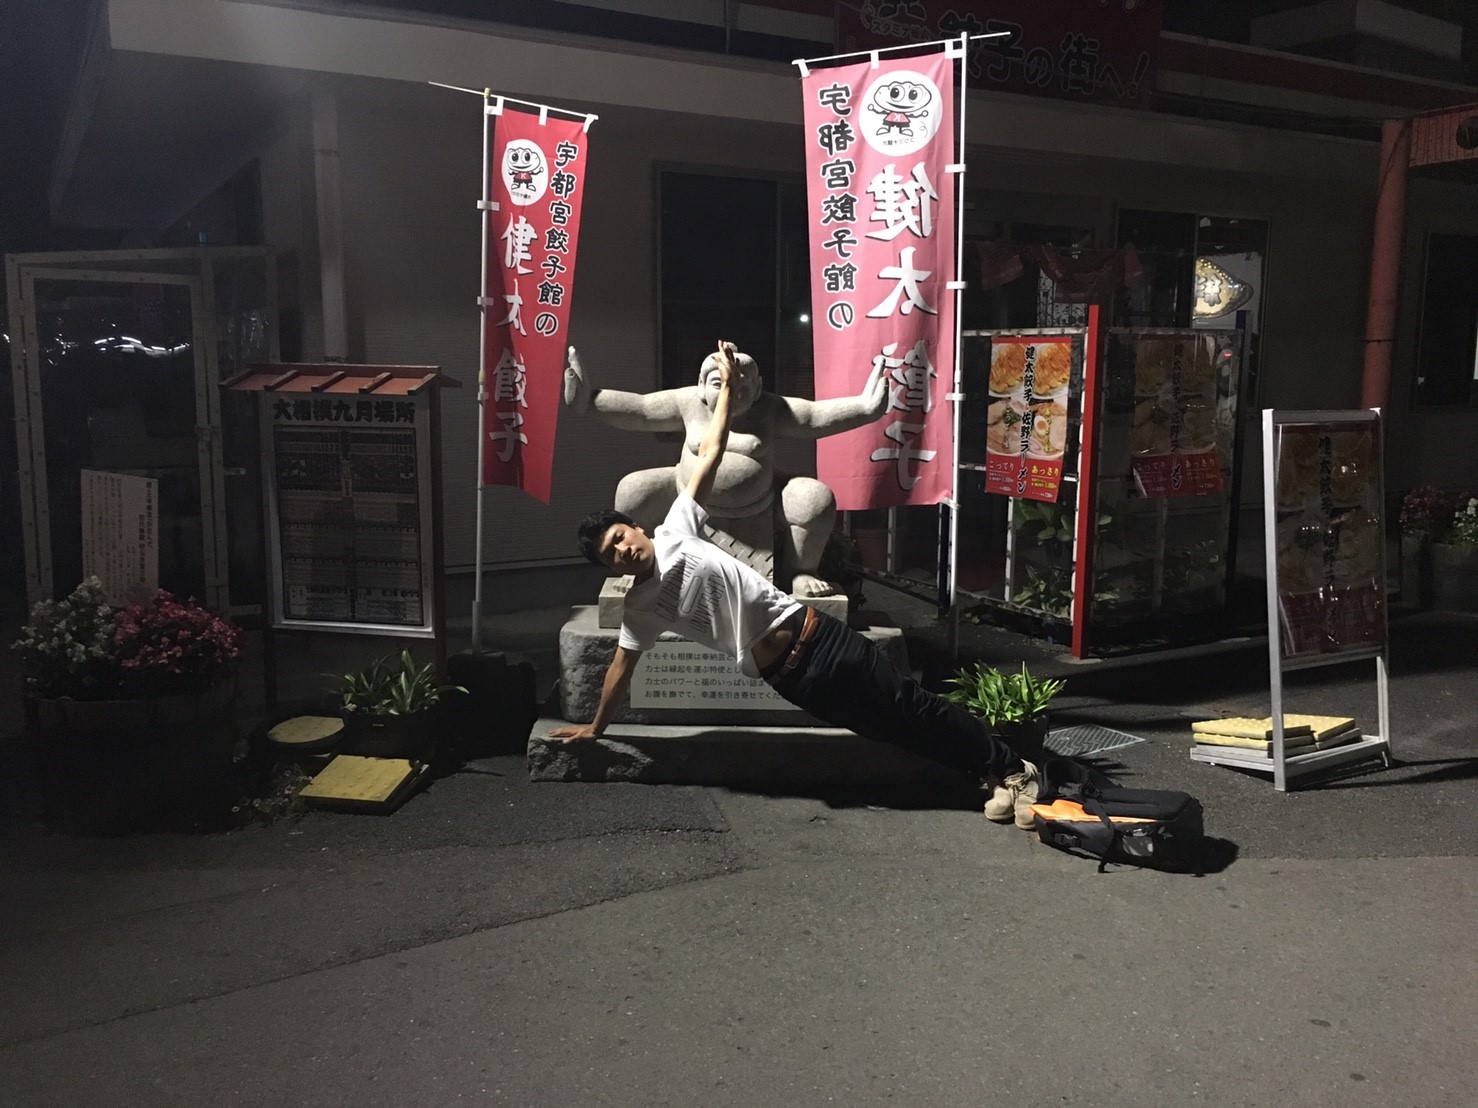
\includegraphics[width=0.6\textwidth]{./section/sasakiLIVE/figures/OgawaPozu.jpg}
  \end{center}
  \caption{飲み会に最後まで残ったものの、未だ有り余る体力の行き場がなく、仕方がなく像の前で体育祭を彷彿とさせる組体操シングルバージョンを披露するオガワマン。誰がこのような結末を予想することができただろうか?}
  \label{fig:TakedaYaruki}
\end{figure}

\begin{figure}[htbp]
  \begin{center}
    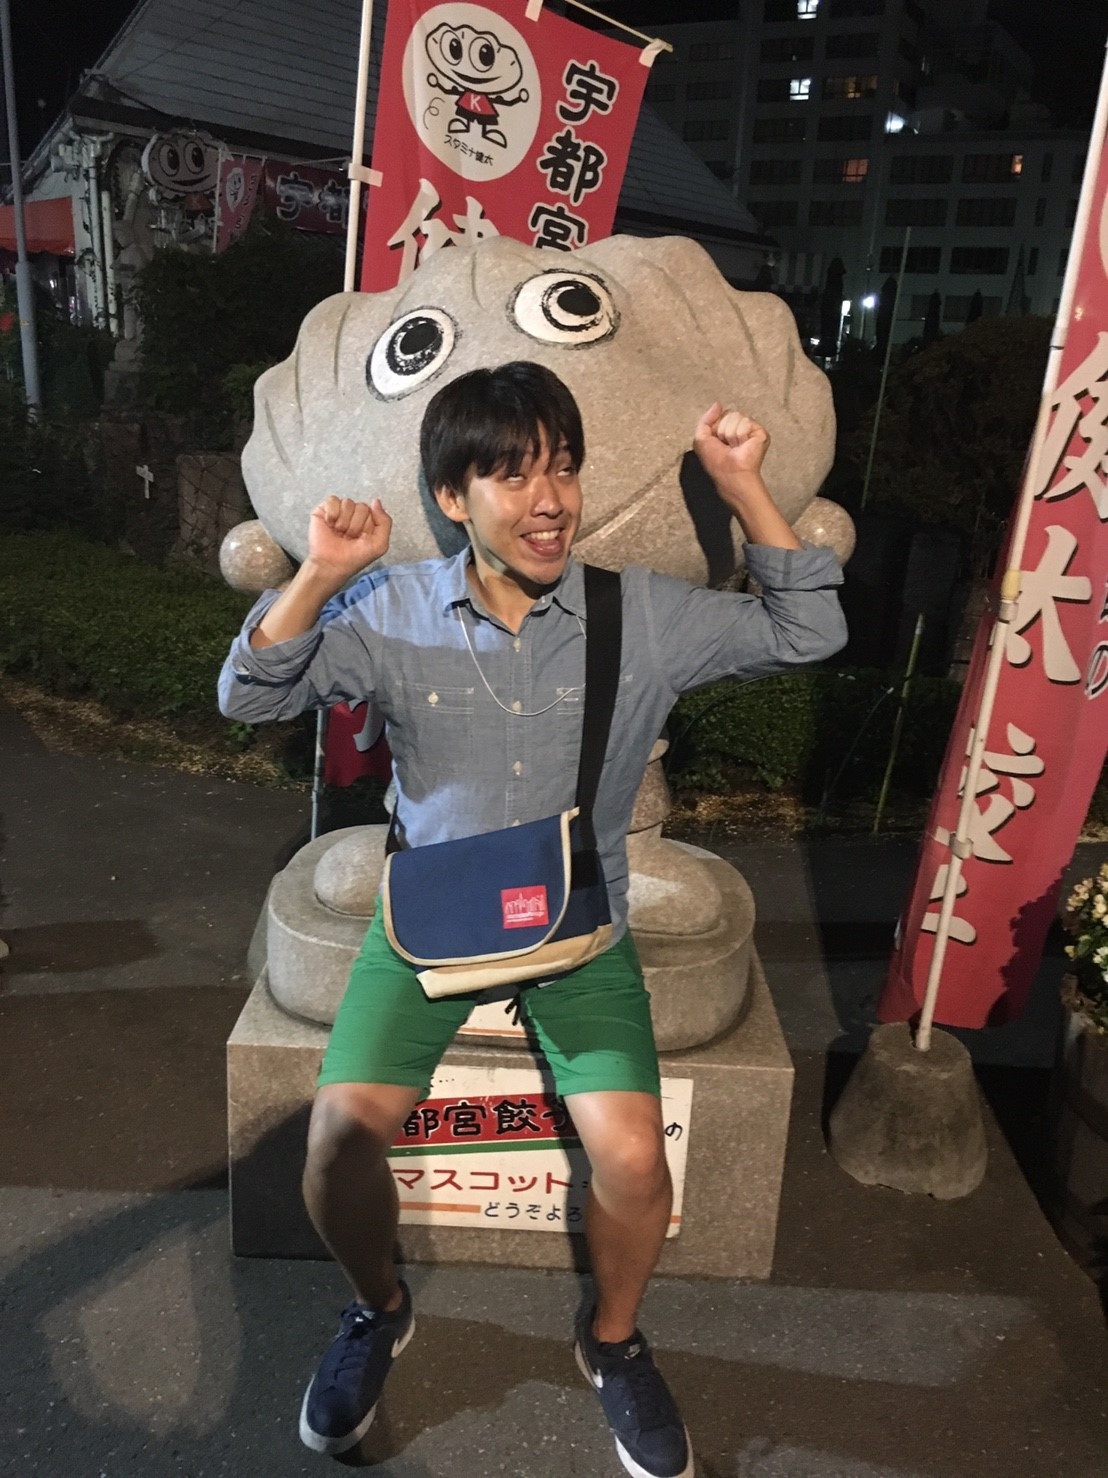
\includegraphics[width=0.5\textwidth]{./section/sasakiLIVE/figures/Gyouza.jpg}
  \end{center}
  \caption{「三次会は!?みんななんで帰ったんや!」という悲痛な叫び。宇都宮名物の餃子マスコット健太の前で、とうとう人間としてのバグが生じた。}
  \label{fig:TakedaYaruki}
\end{figure}


\section{早朝7時起き}
しかし、深夜4時まで動き回ったにも関わらず\footnote{竹田警部に関しては相当量を飲酒をしていた様子である。なにせ一次会でワインを注文したら普通のコップに並々と注がれて出てきたのである。}
、翌日は前準備どおり早朝7時には起床する必要があるのである。
竹田警部健康情報によれば、それは不可能なことであり、だいたい飲んだ翌日は昼間で永眠するのが常であった。
そのため、事前にはカラオケに行くと宣言していたのであるが、それも今ではメンバーがおらず叶わぬ夢となっており、ここでいかにして翌日に起床するかが竹田警部の中での最大の問題となっていた。オガワマン的には起きれるらしく、二人揃って昼間で寝よう、という選択肢は最初から存在していない。
そこで竹田・オガワ両名の相談の結果、ある秘策を思いつくのである。
我々は同じホテルに泊まっているため、まず竹田警部が自分の部屋へと入る。
そして、その部屋の鍵をオガワマンに渡すのである。
そうすることで、翌朝に(正確には数時間後に)竹田警部が起床できるという寸法である。
かくして、数時間の間解散を余儀なくされたのである。

\section{全国瞬時警報システム(Jアラート)}
ここで、すこし本線を脱線し、Jアラートについて簡単に説明する。
Jアラートとは、弾道ミサイル情報、緊急地震速報、津波警報など、対処に時間的余裕のない事態に関する情報を
携帯電話等に配信される緊急速報メール、市町村防災行政無線等により、国から住民まで瞬時に伝達するシステムである。
Jアラートは2004年に整備され、国防力を高めることに一役買っている。
特に、近年では北朝鮮における大陸間弾道ミサイル発射実験の際に、Jアラートによる警報が一躍有名になった。
2017年9月15日には、弾道ミサイルは我が国の北海道地方上空を通過し、襟裳岬の東、約2000キロメートルの太平洋上に落下した。

\begin{figure}[htbp]
  \begin{center}
    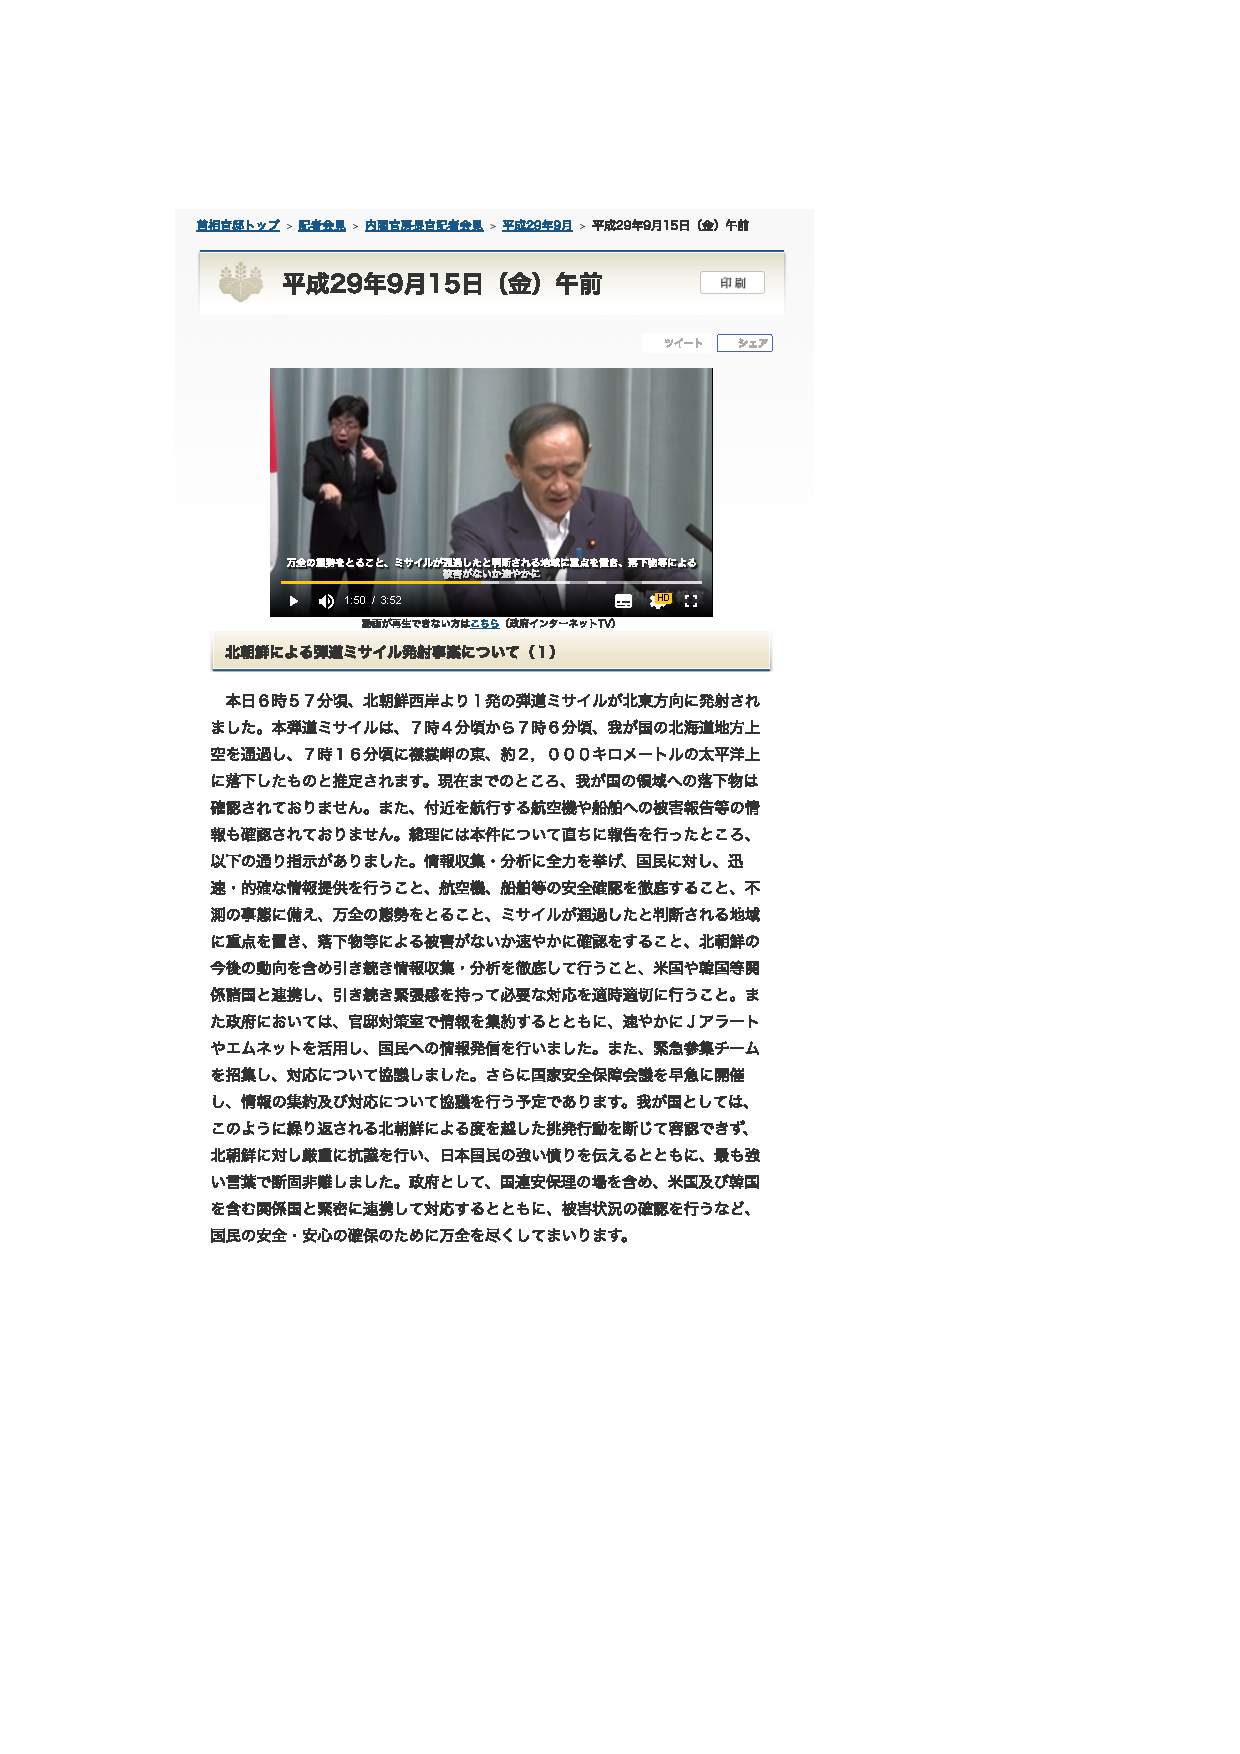
\includegraphics[width=0.5\textwidth]{./section/sasakiLIVE/figures/Jalert.pdf}
  \end{center}
  \caption{2017年9月15日のミサイル発射に関する政府発表。この弾道ミサイル発射は、オガワ直接対決への祝砲となったのか、それとも、、、。}
  \label{fig:Jalert}
\end{figure}

この9月15日明朝とは、野に放たれたポティが憔悴しきった様子でホテルで休息を取っていたのであった。
図\ref{fig:Jalert}に、大陸間弾道ミサイルの発射状況と、竹田氏の睡眠状況を示す。
ここから分かるように、竹田氏は、日本国が国防上の危機に直面しているタイミングで、己の体調の危機を感じ、起きることなく寝ていたのである。
\begin{figure}[htbp]
  \begin{center}
    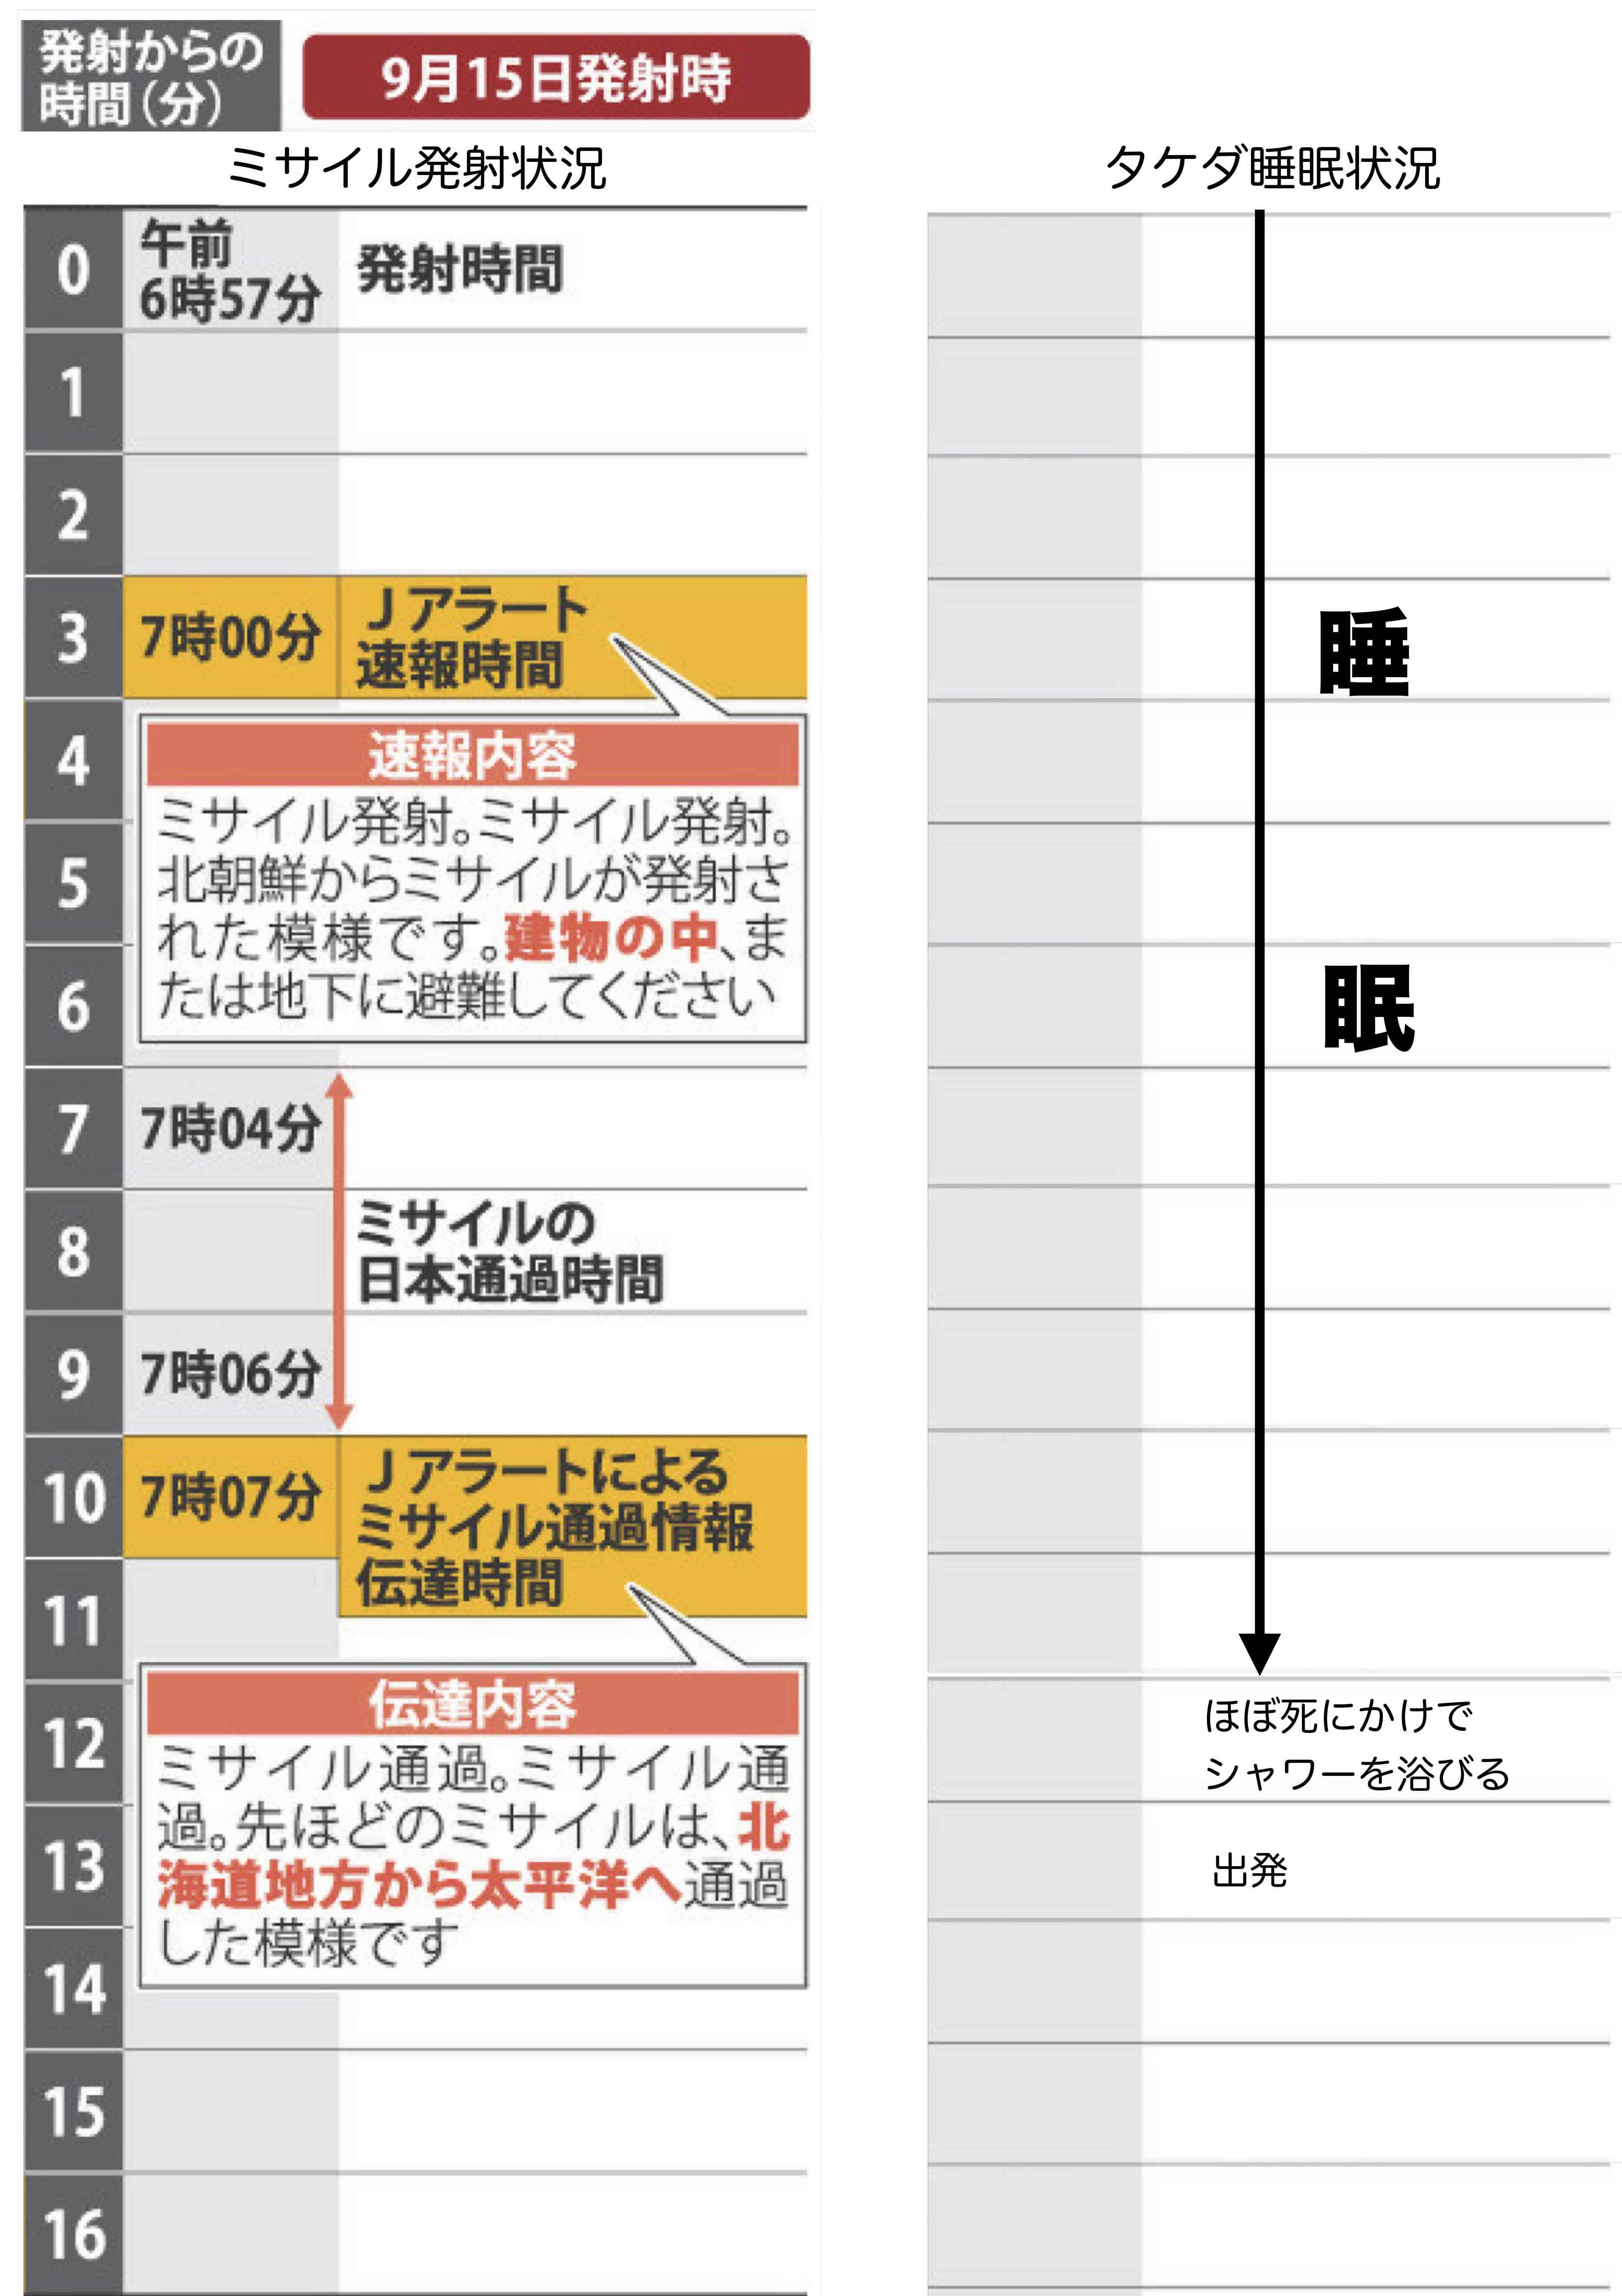
\includegraphics[width=0.5\textwidth]{./section/sasakiLIVE/figures/Suimin.jpg}
  \end{center}
  \caption{北朝鮮が発射したミサイルに関するJアラートの配信状況と、竹田の睡眠状況の相関図。日本の国防の危機にも関わらず、竹田氏は睡眠を優先していたことが伺える。このチャンスを逃したため、竹田氏は未だにJアラートの音色を耳にしたことはない。}
  \label{fig:Jalert}
\end{figure}

\section{全竹田時起床システム(Tアラート)}
その竹田を起床させたのは、全竹田起床システム(Tアラート)である。
Tアラートとは、他人の部屋の鍵を我が物顔で持って帰り、朝になるとその鍵を使って部屋をこじ開け、無理矢理に寝ている竹田を東京へ誘うために無断侵入するオガワにより運用されている。
そのTアラートの効果は絶大であり、Jアラートですら起床しなかった竹田を叩き起こすことに成功したのである。
しかし、竹田は二日酔いなのである。大変なのである。


\section{宇都宮発、東京着}
Tアラートによって起床した竹田警部は、最後の力を振り絞りシャワーを浴び、ホテルを後にしたのである。
しかし、竹田警部は自らの予想通り完全に二日酔いであり、正直電車に乗って良い体調でなかったのである。
完全にランディ・バースが歩く準備が整っており、いつ出塁してもおかしくない状態で2時間ほどの電車は地獄であった。
が、最後の力をもう一度振り絞り、出発前に宇都宮駅で餃子のお土産を買ったのであった。

オガワマンガ竹田警部の体調の悪さへの糾弾に対して、竹田警部は「吐けば治る。納豆巻きたべてポカリ飲んで吐いて、繰り返せば治る」の一点張りであった。
しかし、トイレに行き戻ってきて、またトイレに行きを繰り返すものの一向に体調は回復せず、ランディ・バースが出塁する度に体力が消耗していくのみであった。
ついにたいこ茶屋に到着したわれわれは驚愕の事実を知る。
思っているより全然人が並んでいないのである。おそらく、もはや整理券など不必要なほどに、人はまばらであった。
ほぼ一番乗りで整理券を受け取った我々は、竹田警部の療養のために近くのコンビニに向かった。
しかし時間をかけても休んでも、竹田警部はとうとう体調が戻らないまま、たいこ茶屋海戦の時間を迎えたのである。

\begin{figure}[htbp]
  \begin{center}
    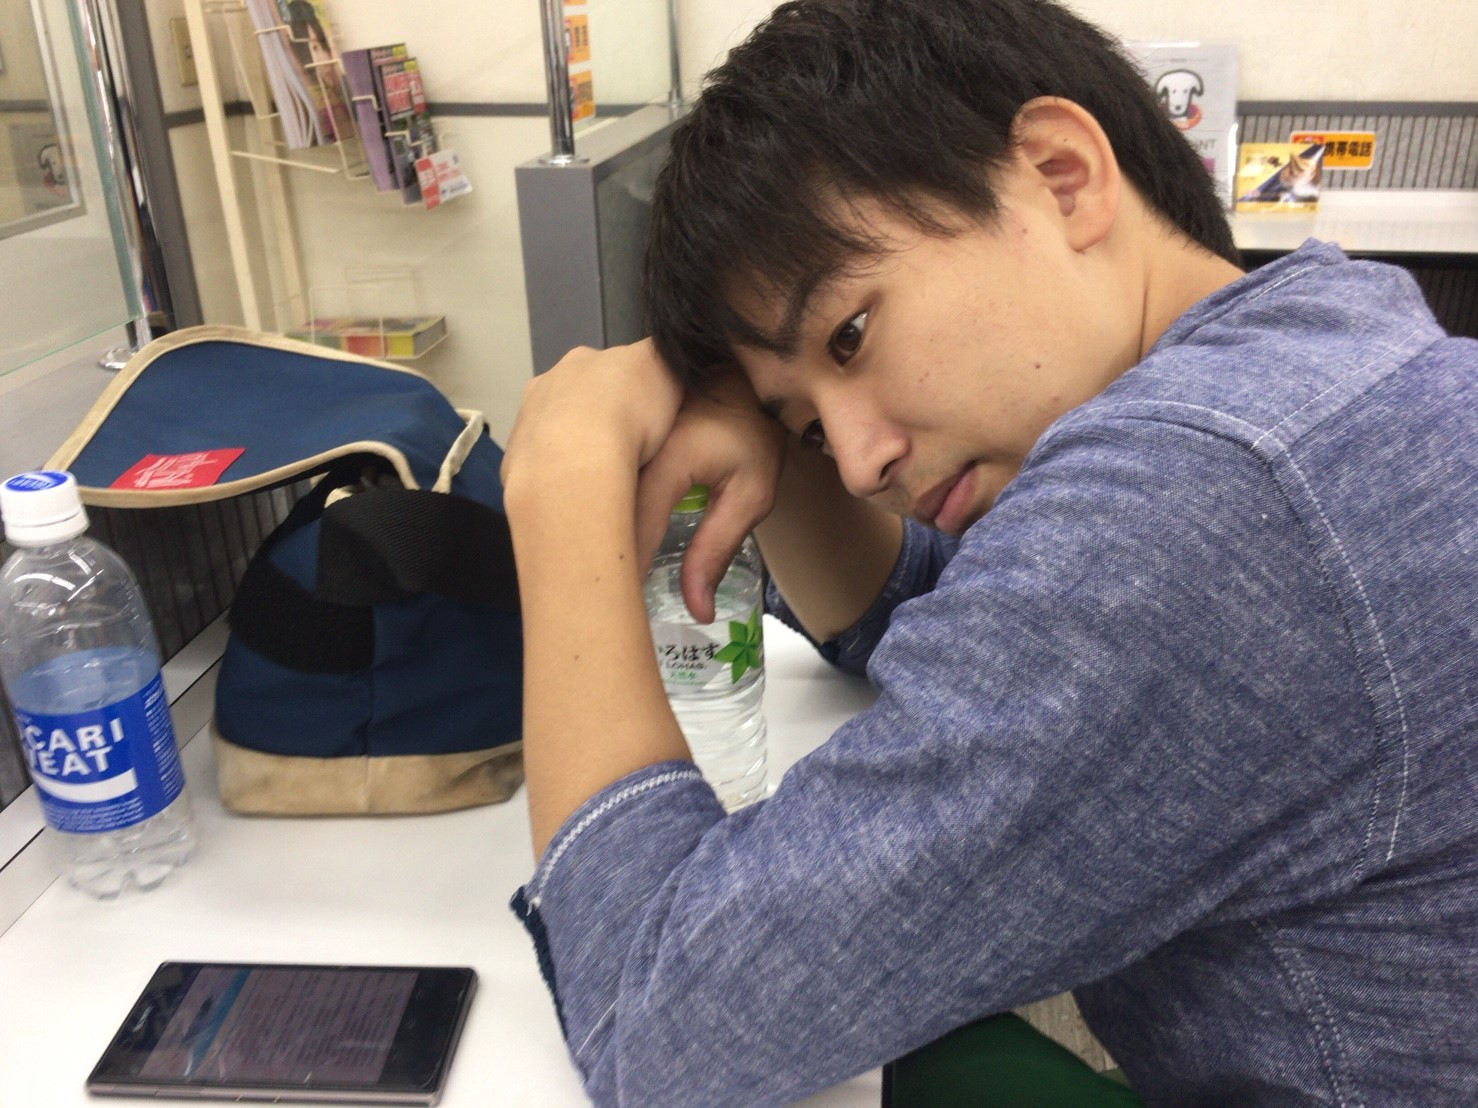
\includegraphics[width=0.5\textwidth]{./section/sasakiLIVE/figures/PoHutsuka.jpg}
  \end{center}
  \caption{完全に二日酔いの状態であり、一向に体力が戻らないままたいこ茶屋周辺のコンビニのイートインで息絶える竹田警部。}
  \label{fig:Jalert}
\end{figure}


\section{たいこ茶屋}
ついに、竹田警部は瀕死のままたいこ茶屋へ入店を果たした。
たいこ茶屋は店の真ん中に様々な海鮮の置いてあるゾーンがあり、またそれとは別に入店時に本日のオススメなる一品も頂くことができる。
完全に食べ放題の夢のパラダイスであり、一日で痛風になってしまいそうなほどの海鮮・醤油摂取量を記録することも容易であろう。
\par
しかし、まず第一の問題点として、本日のオススメの一品が「いくらの醤油漬け」である点だ。
なんとオガワマンはイクラが嫌いなのである。
そして、最大の問題点が、食べ放題の店特有の「食べ残し禁止」という点である。
もちろん自分で食べれる分だけ取って、食べ残しなく食べきれば特段問題はないが、欲張って胃袋の容量以上にお皿に盛り付けようものなら、
罰金が一律500円かかってしまうのである。
\par
竹田警部は食べ放題のゴングが鳴り、本番が始まっても未だ体調が戻らないでいた。
まったく何も食べることができず、かろうじて赤だしを飲んでなんとか酔いを覚まそうとしたり、 トイレにランディ・バースを歩かせに行ったり来たりしていたが、
ついに最後のホイッスルが鳴るまで竹田警部は回復しなかったのである。
そこで問題となってくるのが、食べ残し問題である。
竹田警部は痛恨のミスとして、食べれないのに一丁前に海鮮だけ皿に盛り付けはしていたのである。
また、オガワマンもイクラに苦しんでいた。
これはたいこ茶屋の策略であり、客の食えないものを提供し食べ残させる寸法なのであろう。
\par
我々は、終了の時間が近づいてくる瞬間に、ここが日本国であることを思い出した。
いくら食べ放題といえど、竹田警部の体調の悪さを感じ取ってもらえれば500円の罰金は免除されるであろう。
そう判断した我々は、竹田警部が食べ残した皿をもち返却口へ向かい、渾身の演技でしんどそうな声で「すいません、、、。食べ残したのですが、、、。」
と切り出した。
日本国民がかように体調の悪い人間を放って置くわけがないはずであった。
しかし、ここで竹田警部は最大の誤算をしてしまうのだ。
食べ残した旨を告げた店員を、よく見ると、日本人スタッフではないのである。
海外から日本へ留学して、働いている様子の女性の外国人であった。
そう、ここは日本ではない。日本国民が体調の悪い様子など目には入らない。
彼女の頭の中は、たった一つのルールのみで支配されていた。「食べ残し禁止」。
彼女は無情にも竹田警部に告げたのである。
\begin{center}
「スイマヘーン、500円になりまふぅ」
\end{center}

\section{懲りない男}
かくして500円を払った竹田警部は、命からがらたいこ茶屋から脱出したのである。
が、いまだ体調は戻らず、竹田氏の銭湯へ行きたいと主張した。
銭湯へ行けば体調が戻るはずだ、との信念の元、オガワマンを引き連れスーパー銭湯へ行くことにしたのである。
\par
しかし、その道中にオガワマンは懲りていなかった。
竹田警部が二日酔いで完全にダウンしている最中の犯行であった。
地下鉄に乗って移動しているときに彼は言いました。「あ、財布をさっきのコンビニに忘れてきたかも知れへん。改札出たらちょっと待ってて。」
たいこ茶屋に続く、この日二度目の竹田警部の痛恨のミスは、この歴史的大事件をみすみす逃した点にあろう。
全く何の芸人的反応もできず、改札をでたところでうずくまってオガワマンを待つという醜態をさらすことになった。


